\subsection{Practical considerations} \label{subsec:practical_considerations}% based on scripts/distortions_calc.py
There are two ways we could implement placing objects in the scene:
\begin{enumerate}
    \item Port the object to non-Euclidean geometry and then use the translation given by \autoref{eq:translation},
    \item Translate the object using ordinary Euclidean translation and then port it to non-Euclidean geometry.
\end{enumerate}
We will now shortly discuss both options.

\subsubsection*{Port, then translate}
The first option is undesirable, as it may significantly change the relative positions of objects in the scene.
To see why, let's consider two copies of a 2-dimensional rectangle that we will first port to the spherical geometry, and then translate using the non-Euclidean translation.
The rectangle with vertices $a = (-0.5, -0.7)$, $b = (0.5, -0.7)$, $c = (0.5, 0.5)$, $d = (-0.5, 0.5)$ is ported to spherical geometry using \autoref{eq:elliptic-porting}.
As a result, we obtain points on a unit sphere:
\begin{equation*}
    \begin{split}
         & \mathcal{P}(a) = (-0.441, -0.617, 0.652) \\
         & \mathcal{P}(b) = (0.441, -0.617, 0.652)  \\
         & \mathcal{P}(c) = (0.459, 0.459, 0.760)   \\
         & \mathcal{P}(d) = (-0.459, 0.459, 0.760)
    \end{split}
\end{equation*}
If we were to translate the first copy of the rectangle to point $t_1 = (0.5, 0.5)$ and the second copy to $t _2 = (1.5, 1.7)$ in Euclidean geometry, the two copies should meet at the point $(1, 1)$.

When we perform the translation to point $t_1$ (the corresponding translation target is obtained by porting $t_1$ using \autoref{eq:elliptic-porting}, i.e. the translation target is $q_1 = \mathcal{P}(t_1)$), we get the following vertices:
\begin{equation*}
    \begin{split}
         & \mathcal{P}(a)T_{q_1} =  (-0.014, -0.190, 0.982) \\
         & \mathcal{P}(b)T_{q_1} = (0.761, -0.296, 0.577)   \\
         & \mathcal{P}(c)T_{q_1} = (0.698, 0.698, 0.156)    \\
         & \mathcal{P}(d)T_{q_1} = (-0.110, 0.809, 0.578)
    \end{split}
\end{equation*}
The translation to $t_2$ (with $q_2 = \mathcal{P}(t_2)$) gives
\begin{equation*}
    \begin{split}
         & \mathcal{P}(a)T_{q_2} = (0.709, 0.686, 0.160)   \\
         & \mathcal{P}(b)T_{q_2} = (0.957, -0.031, -0.287) \\
         & \mathcal{P}(c)T_{q_2} = (0.141, 0.099, -0.985)  \\
         & \mathcal{P}(d)T_{q_2} = (-0.117, 0.847, -0.519)
    \end{split}
\end{equation*}
Even though we would expect the third vertex of the first copy of the rectangle to be identical to the first vertex of the second copy, there is a difference between the two.
This effect can be seen in \autoref{fig:spherical-rectangles}.
\begin{figure}[h]
    \centering
    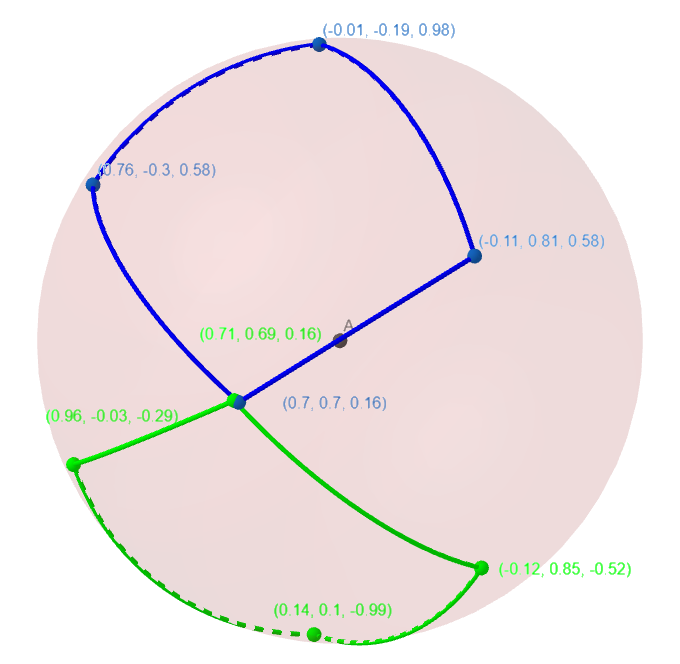
\includegraphics[width=0.6\textwidth]{chapters/theoretical_foundations/sections/non-eudlidean-spaces/resources/spherical-rectangles.png}
    \caption{Rectangles ported onto a sphere and then translated}
    \label{fig:spherical-rectangles}
\end{figure}
The effect is even more visible in the implementation. \autoref{fig:misaligned-wheel} shows how the wheels of the car get misaligned from their wheel arches.
\begin{figure}[h]
    \centering
    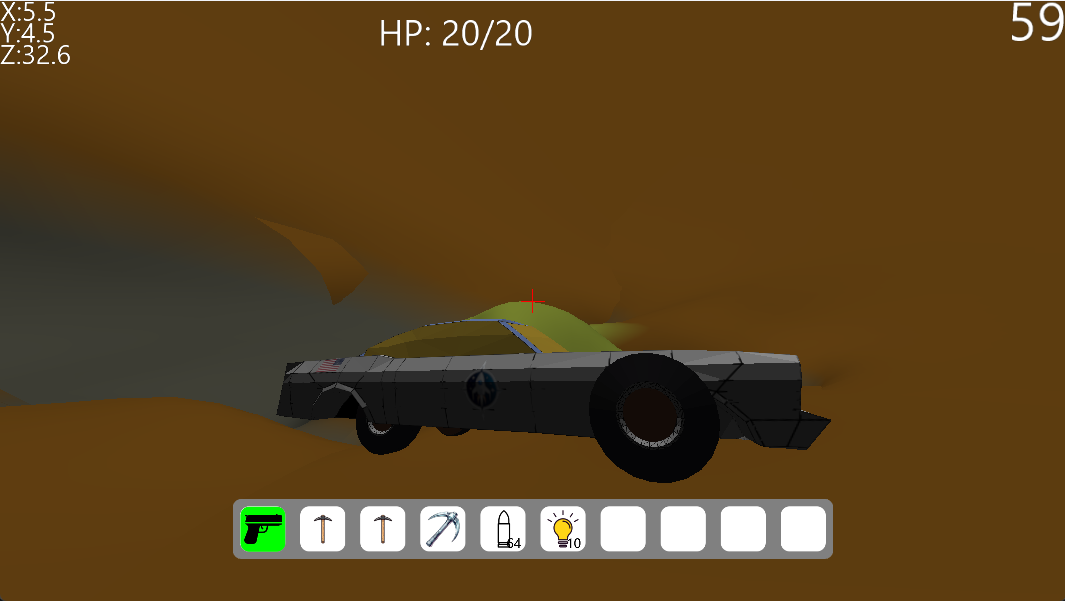
\includegraphics[width=0.6\textwidth]{chapters/theoretical_foundations/sections/non-eudlidean-spaces/resources/misaligned-wheel.png}
    \caption{Non-Euclidean translation causing a misalignment of objects}
    \label{fig:misaligned-wheel}
\end{figure}

\subsubsection*{Translate, then port}
The second option isn't unfortunately free of distortions either.
For example, consider two identical squares of side length $0.5$.
The first one with the bottom-left corner at the point $(0,0)$ and the second one with the corresponding corner at $(0.5, 0.5)$.
After porting to spherical geometry using the \autoref{eq:elliptic-porting}, we get squares with side lengths (listed counter-clockwise starting at the bottom edge):
\begin{equation*}
    0.500, \,
    0.479, \,
    0.479, \,
    0.500
\end{equation*}
for the first square and with side lengths
\begin{equation*}
    0.480, \,
    0.425, \,
    0.425, \,
    0.480
\end{equation*}
for the second square.
The side lengths of the square have been calculated as the lengths of geodesics\footnote{This is the "great-circle distance" equal to $2 \arcsin{(c / 2)}$, where $c$ is the chord length.} between the square's vertices.
As we can see, the side lengths of the ported square are no longer equal to each other, and the distortion increases as the square is farther away from the origin.
This effect can be seen in \autoref{fig:bending-car}.
\begin{figure}[h]
    \centering
    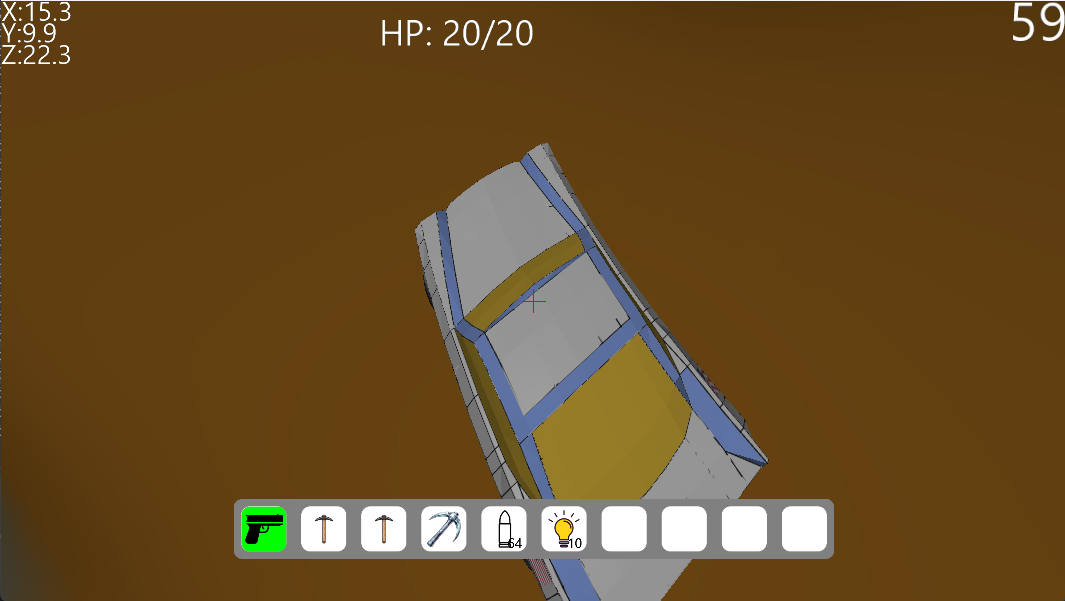
\includegraphics[width=0.6\textwidth]{chapters/theoretical_foundations/sections/non-eudlidean-spaces/resources/bending-car.png}
    \caption{Distrotions caused by porting to spherical space}
    \label{fig:bending-car}
\end{figure}

\subsubsection*{Spherical space}
To minimize the distortions in spherical space we employed the following method.
Due to the periodic nature of the porting given by \autoref{eq:elliptic-porting}, the scene has to be confined inside a 3-dimensional ball of radius $\pi$.
Since the distortions increase as an object is farther from the origin, we decided to split the scene into two physical regions -- balls of radius $\pi / 2$.
Points $p$ in the first ball (centered at the origin) are mapped to spherical geometry using the mapping
\begin{equation} \label{eq:spherical-port-1}
    \mathcal{P}_{E,1}(p) = (p / \lVert p\rVert \sin(\lVert p\rVert), \cos(\lVert p\rVert))
\end{equation}
and points $p$ in the second ball (which is centered at a point $c$) using the formula
\begin{equation}\label{eq:spherical-port-2}
    \mathcal{P}_{E,2}(p) = (p' / \lVert p' \rVert \sin(\lVert p' \rVert), -\cos(\lVert p'\rVert)),
\end{equation}
where $p' = p - c$.
In the 2-dimensional case, the regions become disks with radii of length $\pi$, and the effect of using \autoref{eq:spherical-port-1} and \autoref{eq:spherical-port-2} can be visualized as "wrapping" the first disk on the upper half of a unit sphere, and "wrapping" the second one on the lower half of the sphere.
We should note, that the implementation differs slightly from this description.
More details will be covered in \autoref{sub:teleportation}.

\subsubsection*{Hyperbolic space} \label{subsubsec:practical-considerations-hyperbolic-space}
Dealing with distortions in hyperbolic space requires a more drastic approach because the scene we wished to port was potentially infinite.
The main goal was to keep the distortions as small as possible near the camera and still show the visual aspects indicative of setting the scene in non-Euclidean geometry.
To achieve this, the camera position is fixed at some point close to the origin, e.g. $(0, 1, 0)$.
The movement of the camera is then simulated by moving all of the objects in the scene in the direction opposite to the camera's movement direction.